% Archivo generado automáticamente con los problemas
\section*{Problems}
Sección: 9_Scalar_quantum_electrodynamics
Páginas: 174-175
Contenido:
9.1 Compton scattering in scalar QED.
(a) Calcuate the tree-level matrix elements for (γφ →γφ). Show that the Ward
identity is satisfied.
(b) Calculate the cross section
dσ
d cos θ for this process as a function of the incoming
and outgoing polarizations, ϵin
μ and ϵout
μ , in the center-of-mass frame.
(c) Evaluate
dσ
d cos θ for ϵin
μ polarized in the plane of the scattering, for each ϵout
μ .
(d) Evaluate
dσ
d cos θ for ϵin
μ polarized transverse to the plane of the scattering, for each
ϵout
μ .
(e) Show that when you sum (c) and (d) you get the same thing as having replaced
(ϵin
μ)⋆ϵin
ν with −gμν and (ϵout
μ )⋆ϵout
ν with −gμν.
(f) Should this replacement work for any scattering calculation?

9.2 Consider the following 3-loop diagram for light-by-light scattering:
(9.68)
(a) Approximately how many other diagrams contribute at the same order in pertur-
bation theory? [Hint: you do not need to draw the diagrams.]
156
Scalar quantum electrodynamics
(b) This diagram is not gauge invariant (independent of ξ) by itself. What is the mini-
mal set of diagrams you need to add to this one for the sum to be gauge invariant?
Why should the other diagrams cancel on their own?

9.3 In this problem you will prove the uniqueness of non-Abelian gauge theories by con-
sidering the soft limit when there are multiple scalar fields φi. Suppose these fields
have a mass matrix M (i.e. the mass term in the Lagrangian is L = Mijφ⋆
i φj) and
there are N massless spin-1 particles Aa
μ, a = 1 . . . N we will call gluons. Then the
generic interaction between Aa
μ, φi and φj can be written as Γaμ
ij (p, q) as in Eq. (9.57).
(a) Show that in the soft limit, q ≪p, the charges are now described by a matrix
T a = T a
ij.
(b) For N = 1, show that only if [M, T] = 0 can the theory be consistent. Conclude
that gluons (or the photon) can only couple between particles of the same mass.
(c) Consider Compton scattering, φi(p)Aa
μ(qa) →φj(p′)Ab
ν(qb), in the soft limit
qa, qb ≪p, p′. Evaluate the two diagrams for this process and then show that,
by setting ϵa
μ = qa
μ and ϵb
ν = qb
ν, the interactions are consistent with Lorentz
invariance only if

T a, T b
= 0, assuming nothing else is added.
(d) Show that one can modify this theory with a contact interaction involving
φiφjAa
μAb
ν of the generic form Γabμν
ij

p, qa, qb
so that Lorentz invariance is pre-
served in the soft limit. How must Γabμν
ij
relate to T a
ij? Show also that Γabμν
ij
must
have a pole, for example as (qa + qb)2 →0.
(e) Such a pole indicates a massless particle being exchanged, naturally identified
as a gluon. In this case, the Γabμν
ij
interaction in part (d) can be resolved into a
3-point interaction among gluons, of the form Γabc
μνα

qa, qb, qc
and the Γaμ
ij (p, q)
vertex. Show that if Γabc
μνα itself has no poles, then in the soft limit it can be written
uniquely as Γabc
μνα

qa, qb, qc
= f abc(gμνqα
c + · · · ) for some constants f abc and
work out the · · · . Show that if and only [T a, T b] = if abcT c can the Compton
scattering amplitude be Lorentz invariant in the soft limit. This implies that the
gluons transform in the adjoint representation of a Lie group, as will be discussed
in Chapter 25.

9.4 The soft limit also implies that massless spin-2 particles (gravitons) must have self-
interactions.
(a) To warm up, consider the soft limit of massless spin-1 particles coupled to
scalars (as in scalar QED). Just assuming generic interactions (not the scalar
QED Lagrangian), show that there must be an AAφ⋆φ interaction for Compton
scattering to be Lorentz invariant.
(b) Now consider Compton scattering of gravitons h off scalars. Show that there must
be an hhφφ interaction. Then show that unlike the massless spin-1 case the new
interaction must have a pole at (q1 + q2)2 = 0. This pole should be resolved into
a graviton exchange graph. Derive a relationship between the form of the graviton
self-coupling and the hφφ coupling.

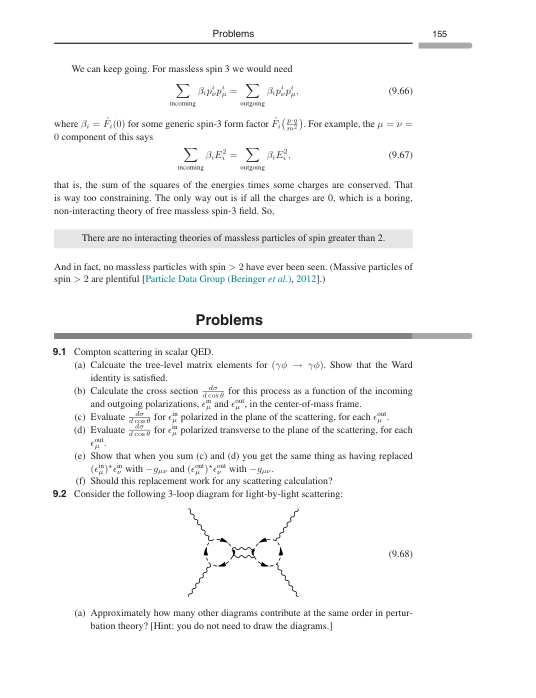
\includegraphics{./figs/9_Scalar_quantum_electrodynamics_page_175.png}

---

